\subsubsection{LSTM Autoencoder}\label{subsec:recautoencoder}
The autoencoder used to pre-train the parameters of the recurrent branch of the RecConvSiameseNet takes MFCCs \& deltas features extracted from each speakers'audio as input, processing the frames one-by-one. The aim here is to extract temporal-wise features from the long-term and short-term relationships between the MFCC \& deltas frames, thanks to the memory capabilities of LSTM layers.

\begin{figure}
	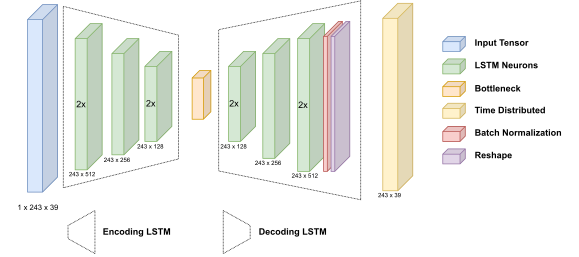
\includegraphics[width=0.5\textwidth]{images/lstm_autoencoder}
	\caption{LSTM Autoencoder}
	\label{fig:lstm_autoencoder}
\end{figure}

Adadelta algorithm has been used with a learning rate of $\eta = 1$ (as suggested by the original paper \cite{adadelta}), $\rho=0.95$ and $\epsilon=10^{-8}$ to train the LSTM autoencoder for 1000 epochs with a batch size of 200~(\vref{fig:lstm_autoencoder_loss}). 

Similar to what we have seen with the convolutional autoencoder, bottleneck activity regularization has been applied, in order to reduce overfitting and make the learned data representations as sparse as possible.

\begin{figure}
	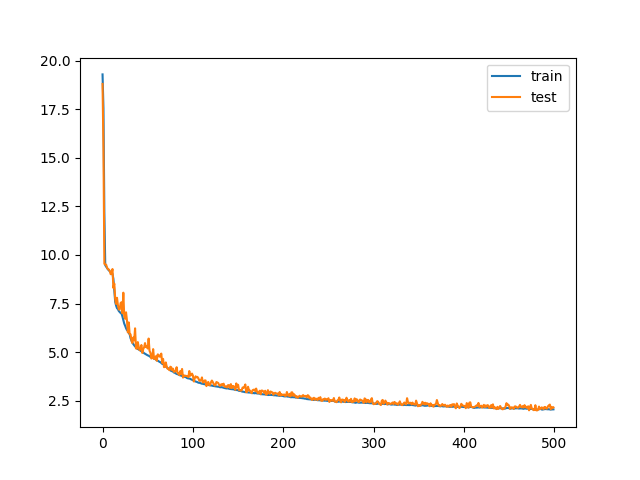
\includegraphics[scale=0.5]{images/lstm_autoencoder_graph.png}
	\caption{LSTM Autoencoder Train/Validation Loss over the first 500 epochs.}
	\label{fig:lstm_autoencoder_loss}
\end{figure}

Diving into the architecture, encoder consists of four LSTM layers with an increasing number of units and a bottleneck of 128 units, as seen in Table~\vref{tab:lstm_encoder}.

\begin{footnotesize}
	\begin{table}
		\centering
		\caption{Parameters of LSTM Encoder}
		\label{tab:lstm_encoder}
		\begin{tabularx}{0.5\textwidth}{XXr}%lMr
			\toprule
			\textbf{Layer Type} & \textbf{Parameters}                                                                   & \textbf{Shape}    \\
			\midrule 
			LSTM               	& Units = 512	                                                                        & (243, 512)        \\[0.25cm] 
			LSTM               	& Units = 512	                                                                        & (243, 512)         \\[0.25cm] 
			LSTM               	& Units = 256	                                                                        & (243, 256)         \\[0.25cm]
			LSTM               	& Units = 128	                                                                        & (243, 128)         \\[0.25cm] 
			Bottleneck          & Dimension = 128	                                                                    &      \\ 
			\bottomrule
		\end{tabularx}
		
	\end{table}
	
\end{footnotesize}

As in the convolutional autoencoder, the decoder is built to a mirrored fashion with respect to the encoder, as we can see in the Table~\vref{tab:lstm_decoder} showing the decoder parameters. A reshape and a time distributed dense layer have been added at the end of the architecture in order to reconstruct the same shape as the fed input. The full LSTM autoencoder architecture is seen in Figure~\vref{fig:lstm_autoencoder}.

\begin{footnotesize}
	\begin{table}
		\centering
		\caption{Parameters of LSTM Decoder}
		\label{tab:lstm_decoder}
		\begin{tabularx}{0.5\textwidth}{XXr}
			\toprule
			\textbf{Layer Type} & \textbf{Parameters}                                                                   & \textbf{Shape}     \\ 
			\midrule
			LSTM               	& Units = 128	                                                                        & (243, 128)         \\[0.25cm] 
			LSTM               	& Units = 256	                                                                        & (243, 256)         \\[0.25cm] 
			LSTM               	& Units = 512	                                                                        & (243, 512)         \\[0.25cm]
			LSTM               	& Units = 512	                                                                        & (243, 512)         \\[0.25cm] 
			Batch Normalization & Features = 1024	                                                                    & (243, 1024)        \\[0.25cm]  
			Time Distributed (Dense)  	& Units = 39				                                                    & (243, 39)          \\
			\bottomrule
		\end{tabularx}
	\end{table}
\end{footnotesize}